\documentclass[a4paper,12pt]{article}
\usepackage[T2A]{fontenc}
\usepackage[utf8x]{inputenc}
\usepackage[english,russian]{babel}
\usepackage{amssymb,amsfonts,amsmath,mathtext}
\usepackage[unicode]{hyperref}
\usepackage{listings}
\usepackage{graphicx}
\usepackage{float}
\graphicspath{{images/}}
\newcommand{\anonsection}[1]{\section*{#1}\addcontentsline{toc}{section}{#1}}

\begin{document}

% Титульный лист

\begin{titlepage}
\newpage

\begin{center}

\textit{Министерство науки и высшего образования Российской Федерации \\ 
Федеральное государственное бюджетное образовательное \\
учреждение высшего образования \\
«Московский государственный технический университет \\
имени Н.Э. Баумана (национальный исследовательский университет)» \\
(МГТУ им. Н.Э. Баумана) \\}
\hrulefill
\end{center}

\vspace{2em}

\begin{flushleft}
ФАКУЛЬТЕТ <<Информатика и системы управления>> \\
\vspace{0.5em}
КАФЕДРА <<Программное обеспечение ЭВМ и информационные технологии>>
\end{flushleft}


\vspace{8em}

\begin{center}
\LARGE Лабораторная работа №8 \\
\end{center}

\vspace{1.5em}

\begin{center}
\textsc{Поиск в словаре}
\end{center}

\vspace{6em}

\begin{center}
Головнев Н.В.

\vspace{4em}

ИУ7-54Б
\end{center}

\vspace{\fill}

\begin{center}
Москва 2019
\end{center}

\end{titlepage}

\tableofcontents

% Введение

\newpage
\anonsection{ВВЕДЕНИЕ}
% Напиши введение

\newpage
\anonsection{ПОСТАНОВКА ЗАДАЧИ}
% Напиши постановку задачи

\newpage
\section{АНАЛИТИЧЕСКАЯ ЧАСТЬ}
\subsection{Описание алгоритма}
\begin{center}
\textbf{Обозначения и терминология}
\end{center}
\quad Обозначим через $\sum^*$ множество всех строк конечной длины, образованных с помощью символов алфавита $\sum$. \textbf{Пустая строка} (empty string) конечной длины, которая обозначается $\varepsilon$, также принадлежит множеству $\sum^*$. Длина строки $x$ обозначается $|x|$. \textbf{Конкатенация} (concatenation) двух строк $x$ и $y$, которая обозначается $xy$, имеет длину $|x| + |y|$ и состоит из символов строки $x$, после которых следуют символы строки $y$.  \\
Говорят, что строка $w$ — \textbf{префикс} (prefix) строки $х$ (обозначается $w \sqsubset x$), если существует такая строка $y \in \sum^*$, что $x = wy$. Если $w \sqsubset x$, то $|w| \leqslant |x|$. Аналогично, строку $w$ называют \textbf{суффиксом} (suffix) строки $x$ (обозначается как $w \sqsupset x$)), если существует такая строка $y \in \sum^*$, что $x = yw$. Из соотношения $w \sqsupset x$ также следует неравенство $|w| \leqslant |x|$. Пустая строка $\varepsilon$ является одновременно и суффиксом, и префиксом любой строки. В качестве примеров префикса и суффикса можно привести $ab \sqsubset abcca$ и $cca \sqsubset abcca$. Для произвольных строк $x$ и $y$ и для любого символа $a$ соотношение $x \sqsupset y$ выполняется тогда и только тогда, когда $xa \sqsupset ya$. Кроме того, отношения $\sqsubset$ и $\sqsupset$ являются транзитивными.
\begin{center}
\textbf{Наивный алгоритм}
\end{center}
Псевдокод наивного алгоритма:\\
1 $n \leftarrow$ длина[$T$]\\
2 $m \leftarrow$ длина[$P$]\\
3 for $s \leftarrow 0$ to $n - m$\\
4 \quad do if $P[1..m] = T[s + 1..s + m]$\\
5 \quad\,\quad then print "Образец обнаружен при сдвиге"\\
\begin{center}
\textbf{Алгоритм Бойера-Мура}
\end{center}
Алгоритм Бойера-Мура последовательно прикладывает образец $P$ к тексту $T$ и проверяет совпадение символов $P$ с прилежащими символами $T$. 3 идеи: просмотр символов слева направо, правило сдвига по плохому символу (стоп-символу) и правило сдвига по хорошему суффиксу. \\
1.Просмотр справа налево.\\
При любом прикладывании $P$ к $T$ алгоритм проверяет совпадение сканированием символов справа налево, начиная с конца, а не слева направо, как в наивном алгоритме.
В случае несовпадения символов, алгоритм продолжает поиск, двигаясь на столько позиций, сколько получается согласно 1-му из 2-х приведенных ниже правил. \\
\\
2.Правило плохого символа.\\
\textbf{Определение}. Для каждого символа алфавита $x$ пусть $R(x)$ - позиция крайне правого вхожения $x$ в $P$. Если $x$ в $P$ не входит, $R(x)$ считается нулем.\\
Предположим, что при некотором сопоставлении $P$ с $T$ крайне правые $n - i$ символов $P$ совпадают со своими парами в $T$, но следующий слева символ $P[i]$ не совпадает со своей парой, скажем, в позиции $k$ строки $T$. \textit{Правило плохого символа} гласит, что $P$ следует сдвинуть вправо на $max{1, i - R[T[k]]}$ позиций. Таким образом, если крайне правое вхождение в $P$ символа $T[k]$ занимает позицию $j < i$ (включая возможность j = 0), то P сдвигается так, чтобы символ $j$ в $P$ поравнялся с символом $k$ в $T$. В противном случае $P$ сдвигается на 1 позицию.\\
\\
3.Правило хорошего суффикса\\
\textbf{Определение}. Для каждого $i$ пусть $L[i]$ - наибольшая позиция, меньшая $n$ и такая, что строка $P[i..n]$ совпадает с суффиксом строки $P[1..L[i]]$. Если такой позиции нет, L[i] считается равным 0. Для каждого $i$ пусть $L^{\prime}$ - наибольшая позиция, меньшая чем $n$ и такая, что $P[i..n]$ совпадает с суффиксом $P[1..L^{\prime}[i]]$, а символ, предшествующий этому суффиксу, не равен $P[i - 1]$. Если такой позиции нет, $L^{\prime}[i]$ считается равным 0.\\ 
Например, если $P = cabdabdab$, то $L[8] = 6$ и $L^{\prime}[8] = 3$.\\
$L[i]$ определяет позицию правого конца крайней правой копии $P[i..n]$, которая сама не является суффиксом $P$, a $L^{\prime}[i]$ - такую же позицию с дополнительнымусиливающим условием, что предшествующий символ не равен $P[i - 1]$. Пожтому в варианте сильного сдвига алгоритма Бойера-Мура, если символ $i - 1$ образца $P$ участвовал в обнаружении несовпадения и $L^{\prime}[i] > 0$, то $P$ сдвигается вправо на $n - L^{\prime}[i]$ позиций. В результате, если правый конец $P$ до сдвига стоял на уровне позиции $k$ в $T$, то на уровне $k$ теперь нужно выровнить позицию $L^{\prime}[i]$.

Псевдокод алгоритма Бойера-Мура:\\
1 $n \leftarrow$ длина[$T$]\\
2 $m \leftarrow$ длина[$P$]\\
3 $L(i) \leftarrow$ таблица суффиксов[$P$]\\
4 $R(x) \leftarrow$ таблица стоп-симолов[$P$] $x \in \sum$\\
5 $k \leftarrow n$\\
6 while $k \leqslant m$\\
7 \quad do $i \leftarrow n$\\
8 \quad\,  $h \leftarrow k$\\
9 \quad\,  while $i > 0$ и $P[i] = T[h]$\\
10\quad\,\quad do $i \leftarrow i - 1$\\
11\quad\,\quad\,  $h \leftarrow h - 1$\\
12\quad\,  if $i = 0$\\
13\quad\,\quad then print "Вхождение найдено"\\
14\quad\,\quad\, увеличить k согласно правилу хорошего суффикса для продолжения работы алгоритма\\
15\quad\,  else\\
16\quad\,\quad then увеличить k на максимальную из величин, задаваемых правилом хорошего суффикса и правилом плохого символа.\\

\begin{center}
\textbf{Алгоритм Кнута-Морриса-Пратта}
\end{center}
В этом алгоритме удается избежать вычисления функции переходов $\delta$, а благодаря использованию вспомогательной функции $\pi$[1..m], которая вычисляется по заданному образцу за время в $\Theta$(m), время сравнения в этом алгоритме равно $\Theta$(n). Вспомогательная функция $\pi$ (также называемая префиксной), предназначенная для какого-нибудь образца, инкапсулирует сведения о том, в какой мере образец совпадает сам с собой после сдвигов. Эта информация позволяет избежать ненужных проверок в простейшем алгоритме поиска подстрок.[\ref{sources:book1}] \\
Более точное определение: \\
\textbf{Префиксной функцией} (prefix function) заданного образца $Р$ [$l$..$m$] называется функция $\pi$ : {1,2,..., $m$} —> {0,1,...,$m$ — 1}, такая что \\
\begin{equation}
\pi[q] = max \{k : k < q \text{ и } P_k \sqsupset P_q\}
\end{equation}
Псевдокод алгоритма Кнута-Морриса-Пратта: \\
1 $n \leftarrow$ длина[$T$] \\
2 $m \leftarrow$ длина[$P$] \\ 
3 $\pi \leftarrow$  префикс-функция($P$) \\
5 for $i \leftarrow 1$ to $n$ \\
6 \quad do while $q > 0$ и $P[q+1] \neq T[i]$ \\ 
7 \qquad\,    do $q \leftarrow \pi[q]$ \\
8 \qquad\,    if $P[q+1] = T[i]$ \\
9 \qquad\,\qquad     then $q \leftarrow q + 1$ \\
10\qquad\,	  if $q = m$ \\
11\qquad\,\qquad     then действие с найденным вхождением \\
12\qquad\,\qquad\,\qquad\   $q \leftarrow \pi[q]$ \\

\newpage
\subsection{Вывод}
% Напиши вывод



\newpage
\section{КОНСТРУКТОРСКАЯ ЧАСТЬ}

\subsection{Разработка алгоритма}
На вход у всех алгоритмов передаются в качестве параметров:
\begin{enumerate}
\item Строка, в которой происходит поиск строки-образца;
\item Длина этой строки; 
\item Строка-образец;
\item Длина строки-образца;
\item Дополнительная память (для простейшего алгоритма поиска она не нужна);
\item Ссылка или указатель на переменную, в которую записывается результат.
\end{enumerate}
Возвращаемое значение: код ошибки (0 в случае успеха, иначе отрицательное значение). \\
Побочные эффекты: изменяется значение переменной результата.

\newpage
\subsection{Схемы алгоритмов}
Ниже представлены схемы алгоритмов поиска в образца в тексте.
% Вставь сюда эти гребаные схемы

\newpage
\subsection{Вывод}
На основе аналитических данных были разработаны требования к разрабатываемым алгоритмам.


\newpage
\section{ТЕХНОЛОГИЧЕСКАЯ ЧАСТЬ}
\subsection{Требования к программному обеспечению}
Программа должна работать на операционной системе Arch Linux. 
Программа должна запускаться из консоли (или терминала) следующей командой:\\
\textit{./app.exe <haystack> <needle>} \\
\textit{app.exe} - само приложение. \textit{<haystack>} - строка текста, в которой будет проводиться поиск строки-образца. \textit{<needle>} - строка-образец.
На выход программа должна печатать позиции для каждого алгоритма, в которых подстрока была обнаружена в строке, а если таких позиций нет, то печатать 0.

\newpage
\subsection{Средства реализации}
Для реализации данных алгоритмов был выбран язык программирования С, компилятор gcc и некоторые функции из библиотеки glibc (memcpy, malloc и тд...). \\

\newpage
\subsection{Листинг кода}
Ниже приведена реализация алгоритма на С.\\
\lstdefinestyle{customc}{
  belowcaptionskip=1\baselineskip,
  breaklines=true,
  frame=L,
  xleftmargin=\parindent,
  language=C,
  showstringspaces=false,
  basicstyle=\footnotesize\ttfamily
}
\lstinputlisting[captionpos=b, caption=\label{listings:listing1}Реализация наивного алгоритма(\ref{images:scheme1}), style=customc]{listing1.c}
\newpage
\lstinputlisting[captionpos=b, caption=\label{listings:listing21}Реализация алгоритма заполнения массива сдвигов (таблицы суффиксов)(\ref{images:scheme1}), style=customc]{listing21.c}
\newpage
\lstinputlisting[captionpos=b, caption=\label{listings:listing22}\text{Реализация алгоритма Бойера-Мура, использующего массив сдвигов}(\ref{images:scheme1}), style=customc]{listing22.c}
\newpage
\lstinputlisting[captionpos=b, caption=\label{listings:listing31}Реализация алгоритма заполнения массива прыжков (таблицы стоп-символов)(\ref{images:scheme1}), style=customc]{listing31.c}
\newpage
\lstinputlisting[captionpos=b, caption=\label{listings:listing32}\text{Реализация алгоритма Бойера-Мура, использующего массив прыжков}(\ref{images:scheme1}), style=customc]{listing32.c}
\newpage
\lstinputlisting[captionpos=b, caption=\label{listings:listing41}Реализация алгоритма заполнения массива префиксов(\ref{images:scheme1}), style=customc]{listing41.c}
\newpage
\lstinputlisting[captionpos=b, caption=\label{listings:listing42}Реализация алгоритма Кнута-Морриса-Прата поиска подстроки в строке(\ref{images:scheme1}), style=customc]{listing42.c}
\newpage

\subsection{Вывод}
Используя язык программирования C, в ходе практической работы были спроектированы и написаны алгоритмы поиска подстроки в строке (стандартный алгоритм, 2 версии алгоритма Бойера-Мура, алгоритм Кнута-Морриса-Пряника).

\newpage
\section{ЭКСПЕРИМЕНТАЛЬНАЯ ЧАСТЬ}
\subsection{Характеристики аппаратного и программного обеспечения}
% Часть которую никогда нельзя менять
Тестирование приложения проводилось на машине со следующими характеристиками:\\
\begin{itemize}
\item Процессор Intel® Core™ i7-7700HQ;
\item Оперативная память 16 ГБ;
\item Операционная система - Arch Linux с рабочим окружением Cinnamon.
\end{itemize}

\newpage
\subsection{Примеры работы}
На Рис. \ref{images:example}, предсавленном ниже, демонстрируется работа приложения. Запуск приложения осуществляется из эмулятора терминала в Arch Linux. На вход подается 
строка, в которой происходит поиск строка-образец, и сама строка-образец.
\begin{figure}[h]
\center{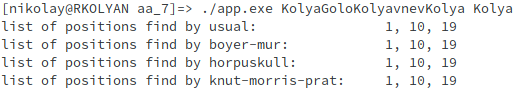
\includegraphics[scale=0.75]{example.png}}
\caption{Пример работы приложения}
\label{images:example}
\end{figure}

\newpage
\subsection{Оценка затрачиваемой памяти}
1)Размер памяти (в байтах) $M$, необходимый для работы алгоритма стандартного алгоритма:\\
\begin{equation}
M =  T * (L_1 + L_2) + S
\end{equation}
где:\\
$T$ - количество байт, выделенное под 1 символ,\\
$L_1$ - длина 1-й строки (основной строки),\\
$L_2$ - длина 2-й строки (строки-образца),\\
$S$ - память, используемая в стеке для обеспечения работы алгоритма. \\

2)Размер памяти (в байтах) $M$, необходимый для работы алгоритма алгоритма Бойера-Мура, использующий массив прыжков (таблицу стоп символов):\\
\begin{equation}
M = T_1 * (L_1 + L_2) + \vert V \vert * T_2 + S
\end{equation} 
где:\\
$T_1$ - количество байт, выделенное под 1 символ,\\
$T_2$ - количество байт, выделенное под 1 элемент массива прыжков,\\
$\vert V \vert$ - количество символов в используемом алфавите V,\\
$L_1$ - длина 1-й строки (основной строки),\\
$L_2$ - длина 2-й строки (строки-образца),\\
$S$ - память, используемая в стеке для обеспечения работы алгоритма. \\

3)Размер памяти (в байтах) $M$, необходимый для работы алгоритма алгоритма Бойера-Мура, использующий массив сдвигов (таблицу суффиксов):\\
\begin{equation}
M = T_1 * (L_1 + L_2) + (L_2 + 1) * T_2 + S
\end{equation}
где:\\
$T_1$ - количество байт, выделенное под 1 символ,\\
$T_2$ - количество байт, выделенное под 1 элемент массива сдвигов,\\
$L_1$ - длина 1-й строки (основной строки),\\
$L_2$ - длина 2-й строки (строки-образца),\\
$S$ - память, используемая в стеке для обеспечения работы алгоритма. \\

4)Размер памяти (в байтах) $M$, необходимый для работы алгоритма алгоритма Кнута-Морриса-Прата:\\
\begin{equation}
M = T_1 * (L_1 + L_2) + L_2 * T_2 + S
\end{equation}
где:\\
$T_1$ - количество байт, выделенное под 1 символ,\\
$T_2$ - количество байт, выделенное под 1 элемент массива префиксов,\\
$L_1$ - длина 1-й строки (основной строки),\\
$L_2$ - длина 2-й строки (строки-образца),\\
$S$ - память, используемая в стеке для обеспечения работы алгоритма. \\

\newpage
\subsection{Вывод}
В ходе экспериментальной части работы было протестирована работа приложения. Также была проведенка оценка затрачиваемой памяти реализованных алгоритмов. Самым худшим по памяти является алгоритм Бойера-Мура, самым лучшим по памяти - стандартный.

\newpage
\anonsection{ЗАКЛЮЧЕНИЕ}
Поиск в словаре в основном нужен для проверки орфографии в редакторах текста. Также, он ускоряет написание программ в интегрированных средствах разработки путем автоподставления слов (переменных, функций и тд).

\newpage
\anonsection{СПИСОК ИСТОЧНИКОВ}
\begin{itemize}
\item \label{site:wikipedia}https://ru.wikipedia.org/wiki/
\item \label{site:habr}https://habr.com/ru/post/422085/
\end{itemize}

\end{document}
